\documentclass[11pt,a4paper]{article}
%%%%%%%%%%%%%%%%%%%%%%%%% Credit %%%%%%%%%%%%%%%%%%%%%%%%

% template ini dibuat oleh martin.manullang@if.itera.ac.id untuk dipergunakan oleh seluruh sivitas akademik itera.

%%%%%%%%%%%%%%%%%%%%%%%%% PACKAGE starts HERE %%%%%%%%%%%%%%%%%%%%%%%%
\usepackage{graphicx}
\usepackage{caption}
\usepackage[expansion=false]{microtype}
\captionsetup[table]{name=Tabel}
\captionsetup[figure]{name=Gambar}
\usepackage{tabulary}
\usepackage{minted}
% \usepackage{amsmath}
\usepackage{fancyhdr}
% \usepackage{amssymb}
% \usepackage{amsthm}
\usepackage{placeins}
% \usepackage{amsfonts}
\usepackage{graphicx}
\usepackage[all]{xy}
\usepackage{tikz}
\usepackage{verbatim}
\usepackage[left=2cm,right=2cm,top=3cm,bottom=2.5cm]{geometry}
\usepackage{hyperref}
\hypersetup{
    colorlinks,
    linkcolor={red!50!black},
    citecolor={blue!50!black},
    urlcolor={blue!80!black}
}
\usepackage{caption}
\usepackage{subcaption}
\usepackage{multirow}
\usepackage{psfrag}
\usepackage[T1]{fontenc}
\usepackage[scaled]{beramono}
% Enable inserting code into the document
\usepackage{listings}
\usepackage{xcolor} 
% custom color & style for listing
\definecolor{codegreen}{rgb}{0,0.6,0}
\definecolor{codegray}{rgb}{0.5,0.5,0.5}
\definecolor{codepurple}{rgb}{0.58,0,0.82}
\definecolor{backcolour}{rgb}{0.95,0.95,0.92}
\definecolor{LightGray}{gray}{0.9}
\lstdefinestyle{mystyle}{
backgroundcolor=\color{backcolour},   
commentstyle=\color{green},
keywordstyle=\color{codegreen},
numberstyle=\tiny\color{codegray},
stringstyle=\color{codepurple},
basicstyle=\ttfamily\footnotesize,
breakatwhitespace=false,         
breaklines=true,                 
captionpos=b,                    
keepspaces=true,                 
numbers=left,                    
numbersep=5pt,                  
showspaces=false,                
showstringspaces=false,
showtabs=false,                  
tabsize=2
}
\lstset{style=mystyle}
\renewcommand{\lstlistingname}{Kode}
%%%%%%%%%%%%%%%%%%%%%%%%% PACKAGE ends HERE %%%%%%%%%%%%%%%%%%%%%%%%


%%%%%%%%%%%%%%%%%%%%%%%%% Data Diri %%%%%%%%%%%%%%%%%%%%%%%%
\newcommand{\studentlist}{
    \item \textbf{Joshua Palti Sinaga (122140141)}
    \item \textbf{Rustian Afencius Marbun (122140155)}
}
\newcommand{\course}{\textbf{Pembelajaran Mendalam (IF25-40401)}}
\newcommand{\assignment}{\textbf{Tugas Eksplorasi}}

%%%%%%%%%%%%%%%%%%% using theorem style %%%%%%%%%%%%%%%%%%%%
\newtheorem{thm}{Theorem}
\newtheorem{lem}[thm]{Lemma}
\newtheorem{defn}[thm]{Definition}
\newtheorem{exa}[thm]{Example}
\newtheorem{rem}[thm]{Remark}
\newtheorem{coro}[thm]{Corollary}
\newtheorem{quest}{Question}[section]
%%%%%%%%%%%%%%%%%%%%%%%%%%%%%%%%%%%%%%%%
\usepackage{lipsum}%% a garbage package you don't need except to create examples.
\pagestyle{fancy}
\lhead{Joshua Palti Sinaga (122140141), Rustian Afencius Marbun (122140155)}
\rhead{ \thepage}
\cfoot{\textbf{Tugas Eksplorasi: Eksperimen Arsitektur ResNet-34}}
\renewcommand{\headrulewidth}{0.4pt}
\renewcommand{\footrulewidth}{0.4pt}

%%%%%%%%%%%%%%  Shortcut for usual set of numbers  %%%%%%%%%%%

\newcommand{\N}{\mathbb{N}}
\newcommand{\Z}{\mathbb{Z}}
\newcommand{\Q}{\mathbb{Q}}
\newcommand{\R}{\mathbb{R}}
\newcommand{\C}{\mathbb{C}}
\setlength\headheight{14pt}

%%%%%%%%%%%%%%%%%%%%%%%%%%%%%%%%%%%%%%%%%%%%%%%%%%%%%%%555
\begin{document}
\thispagestyle{empty}
\begin{center}

\includegraphics[scale = 0.15]{Figure/ifitera-header.png}
\vspace{0.1cm}
\end{center}
\noindent
\rule{17cm}{0.2cm}\\[0.3cm]
Mata Kuliah: \course \hfill Tugas: \assignment\\[0.1cm]
{Kelompok NgodingDiKertas:} \hfill Tanggal: \textbf{29 September 2025}
\begin{enumerate}
    \studentlist
\end{enumerate}
\rule{17cm}{0.05cm}
\vspace{0.1cm}



%%%%%%%%%%%%%%%%%%%%%%%%%%%%%%%%%%%%%%%%%%%%% BODY DOCUMENT %%%%%%%%%%%%%%%%%%%%%%%%%%%%%%%%%%%%%%%%%%%%%

\begin{center}
\section*{Eksperimen Arsitektur ResNet-34}
\end{center}
\vspace{0.5cm}
\section{Tahap 1: Analisis Performa Model Dasar (Plain Network)}
\subsection{Arsitektur Plain-34}
Plain-34 adalah arsitektur yang mirip dengan ResNet-34 tanpa skip connection, memiliki 34 layer untuk memproses gambar 224x224 pixels. Arsitektur dimulai dengan convolutional layer 7x7 (stride 2, 64 channel), batch normalization, ReLU, dan max pooling 3x3 (stride 2). Kemudian terdapat empat stage: Stage 1 (3 block, 64 channel), Stage 2 (4 block, 128 channel), Stage 3 (6 block, 256 channel), dan Stage 4 (3 block, 512 channel), dengan stride 2 pada block pertama di stage 2-4. Setiap Plain Block terdiri dari dua layer Conv 3x3 + BatchNorm + ReLU. Arsitektur diakhiri dengan global average pooling dan fully connected layer untuk 5 kelas. Perbedaan utama dengan ResNet-34 adalah output block langsung diproses tanpa dijumlahkan dengan input (tidak ada skip connection).

\subsection{Konfigurasi Pelatihan}
\begin{table}[h]
\centering
\caption{Hyperparameter Training}
\begin{tabular}{|l|l|}
\hline
\textbf{Parameter} & \textbf{Nilai} \\ \hline
Learning Rate & 0.001 (1e-3) \\ \hline
Batch Size (Training) & 32 \\ \hline
Batch Size (Validation) & 64 \\ \hline
Optimizer & SGD \\ \hline
Jumlah Epoch & 8 \\ \hline
Loss Function & CrossEntropyLoss \\ \hline
\end{tabular}
\end{table}

\subsection{Implementasi}
Implementasi menggunakan PyTorch dengan PlainBlock yang terdiri dari dua Conv3x3-BN-ReLU secara berurutan tanpa skip connection. Dataset 5 kelas makanan Indonesia dibagi 80\% training dan 20\% validation. Model dilatih 8 epoch dengan monitoring loss dan accuracy.

\subsection{Hasil Pelatihan}
Hasil menunjukkan performa rendah dengan 21.29M parameter. Training loss turun konsisten (1.609→1.591), validation loss stabil di ~1.57. Accuracy sangat rendah: training 22.7\%, validation 24.7\%, best validation 27.1\% (epoch 5), hanya sedikit di atas random guessing (20\%). Overfitting monitor menunjukkan nilai negatif setelah epoch 2, mengindikasikan model menghafal training data tanpa generalisasi baik.
\begin{figure}[h]
\centering
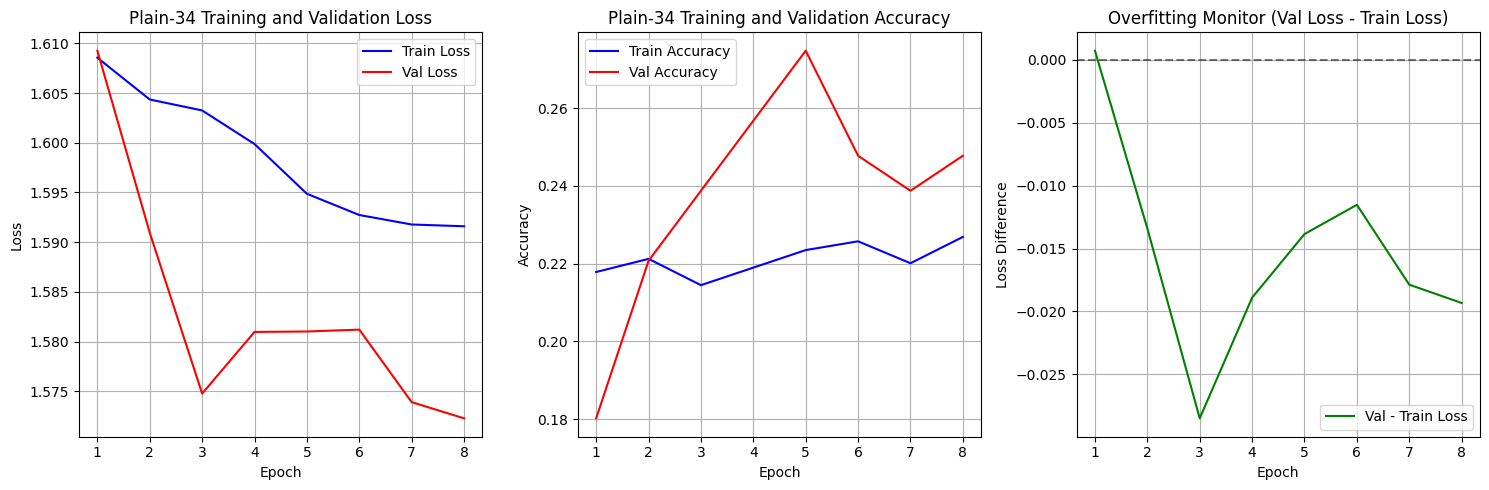
\includegraphics[width=0.95\textwidth]{Figure/plainnet34.png}
\caption{Grafik Training dan Validation Plain-34}
\label{fig:plain34}
\end{figure}
\begin{table}[h]
\centering
\caption{Ringkasan Hasil Training Plain-34}
\begin{tabular}{|l|c|c|}
\hline
\textbf{Metrik} & \textbf{Training} & \textbf{Validation} \\ \hline
Final Loss & ~1.591 & ~1.573 \\ \hline
Final Accuracy & ~22.7\% & ~24.7\% \\ \hline
Best Val Accuracy & - & ~27.1\% (epoch 5) \\ \hline
Total Parameters & \multicolumn{2}{c|}{21,289,989} \\ \hline
\end{tabular}
\end{table}
\subsection{Analisis}
Performa Plain-34 sangat rendah (max 27\%) menunjukkan masalah degradasi pada jaringan dalam tanpa skip connection. 
Dengan 34 layer, gradient mengalami vanishing gradient problem karena perkalian berulang dengan nilai kecil saat backpropagation, 
menyebabkan layer awal tidak ter-update efektif. Overfitting terlihat dari validation loss lebih rendah dari training loss setelah epoch 2, 
dan validation accuracy turun setelah puncak di epoch 5.

\section{Tahap 2: Implementasi Residual Connection (ResNet-34)}
\subsection{Modifikasi Arsitektur}
ResNet-34 identik dengan Plain-34 namun menambahkan skip connection pada setiap block. Perbedaan kunci: Plain-34 menggunakan output = ReLU(Conv2(ReLU(Conv1(x)))), sedangkan ResNet-34 menggunakan output = ReLU(Conv2(ReLU(Conv1(x))) + x). Penambahan input x (skip connection) menciptakan "jalan pintas" untuk aliran gradient. Residual block menyimpan input sebagai identity, memproses melalui Conv-BN-ReLU-Conv-BN menghasilkan F(x), lalu menjumlahkan F(x) + x sebelum ReLU final. Model hanya perlu belajar residual F(x) = H(x) - x, bukan transformasi penuh H(x). Untuk dimensi berbeda, digunakan downsample layer (Conv 1x1). Semua konfigurasi lain sama dengan Plain-34 untuk perbandingan fair.

\subsection{Implementasi}
Implementasi ResNetBlock memodifikasi forward function dengan menyimpan input sebagai identity, memproses melalui Conv-BN-ReLU-Conv-BN, lalu menjumlahkan hasil dengan identity (skip connection: out + identity) sebelum ReLU final. Downsample digunakan jika dimensi berbeda.

\subsection{Hasil Pelatihan}
ResNet-34 menunjukkan peningkatan signifikan dengan parameter sama (21.29M). Loss turun smooth: training 1.605→1.538, validation 1.605→1.516. Accuracy meningkat drastis: training 34.4\%, validation 30.0\%, best validation 44.7\% (epoch 6), jauh melampaui Plain-34. Learning curve konsisten naik hingga epoch 6. Overfitting lebih terkontrol dengan loss difference stabil, menunjukkan skip connection membantu regularisasi implisit.
\begin{figure}[h]
\centering
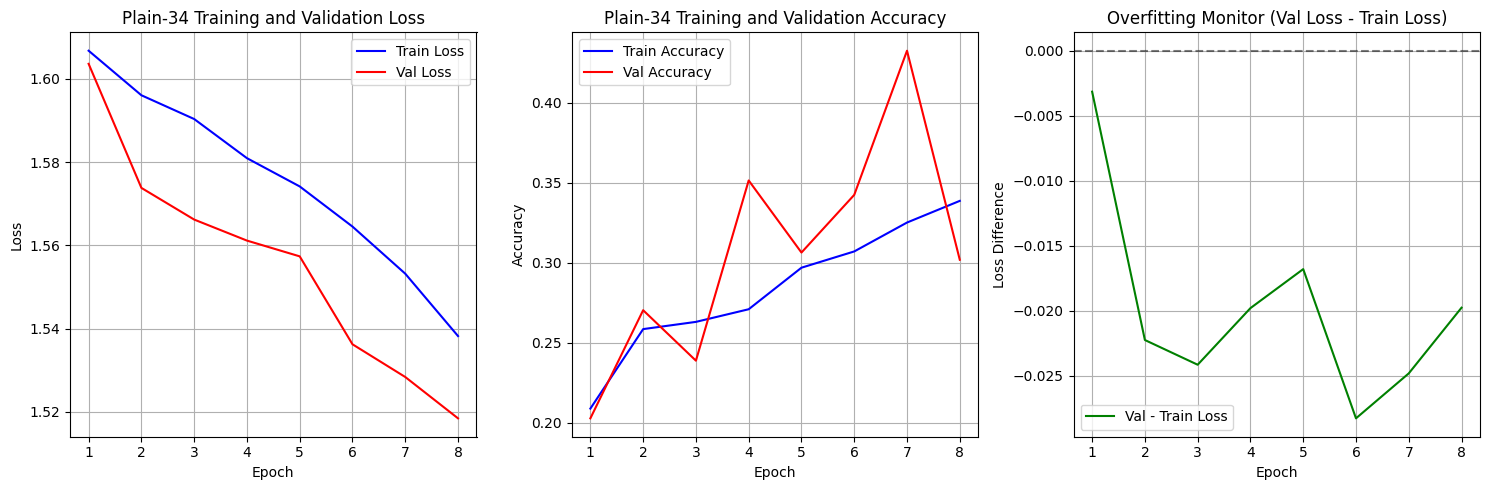
\includegraphics[width=0.95\textwidth]{Figure/resnet34.png}
\caption{Grafik Training dan Validation ResNet-34}
\label{fig:resnet34}
\end{figure}
\begin{table}[h]
\centering
\caption{Ringkasan Hasil Training ResNet-34}
\begin{tabular}{|l|c|c|}
\hline
\textbf{Metrik} & \textbf{Training} & \textbf{Validation} \\ \hline
Final Loss & ~1.538 & ~1.516 \\ \hline
Final Accuracy & ~34.4\% & ~30.0\% \\ \hline
Best Val Accuracy & - & ~44.7\% (epoch 6) \\ \hline
Total Parameters & \multicolumn{2}{c|}{21,289,989} \\ \hline
\end{tabular}
\end{table}
\subsection{Perbandingan dengan Plain-34}
\begin{table}[h]
\centering
\caption{Perbandingan Plain-34 vs ResNet-34}
\begin{tabular}{|l|c|c|c|}
\hline
\textbf{Metrik} & \textbf{Plain-34} & \textbf{ResNet-34} & \textbf{Improvement} \\ \hline
Best Val Accuracy & 27.1\% & 44.7\% & +17.6\% \\ \hline
Final Val Accuracy & 24.7\% & 30.0\% & +5.3\% \\ \hline
Final Train Accuracy & 22.7\% & 34.4\% & +11.7\% \\ \hline
Final Val Loss & 1.573 & 1.516 & -0.057 \\ \hline
Final Train Loss & 1.591 & 1.538 & -0.053 \\ \hline
Total Parameters & 21.29M & 21.29M & Sama \\ \hline
\end{tabular}
\end{table}

Skip connection memberikan dampak signifikan. Best validation accuracy meningkat 64.9\% (27.1\%→44.7\%), final validation accuracy +5.3\%, training accuracy +11.7\%. Loss turun: validation -0.057, training -0.053. Yang penting, peningkatan ini dicapai dengan parameter sama persis (21.29M), membuktikan efektivitas murni dari skip connection. ResNet-34 menunjukkan konvergensi lebih cepat, kurva smooth dan stabil, berbeda dengan Plain-34 yang stagnan dan fluktuatif.

\subsection{Analisis Kritis}
Tiga faktor menjelaskan efektivitas skip connection: (1) Mengatasi vanishing gradient dengan menyediakan "jalan pintas" langsung untuk gradient flow, memastikan layer awal tetap ter-update efektif. (2) Mempermudah optimisasi dengan mengubah target pembelajaran dari H(x) menjadi residual F(x) = H(x) - x. Model bisa mudah belajar identity mapping jika layer tidak diperlukan (F(x)$\approx$0). (3) Memecahkan masalah degradasi, memungkinkan jaringan sangat dalam tanpa penurunan performa.\\\\Bukti empiris kuat: dengan parameter sama, ResNet-34 64.9\% lebih baik, konvergensi lebih cepat dan stabil. Kesimpulan: skip connection adalah inovasi sederhana namun revolusioner, mengatasi masalah fundamental deep learning (vanishing gradient dan degradasi) dengan hanya operasi penjumlahan.


\section{Tahap 3: Eksperimen Modifikasi Arsitektur ResNet-34}
\subsection{Pemilihan Modifikasi}
Sebutkan DUA modifikasi yang dipilih

\subsection{Justifikasi Pemilihan}
Berikan justifikasi kuat mengapa memilih kedua modifikasi tersebut

\subsection{Modifikasi 1: [Nama Modifikasi]}
\subsubsection{Deskripsi Arsitektur}
% Jelaskan detail arsitektur modifikasi pertama

\subsubsection{Implementasi}
% Jelaskan detail implementasi

\subsubsection{Hasil Pelatihan}
% Tampilkan hasil pelatihan dengan format yang konsisten

\subsubsection{Analisis}
% Analisis hasil

\subsection{Modifikasi 2: [Nama Modifikasi]}
\subsubsection{Deskripsi Arsitektur}
% Jelaskan detail arsitektur modifikasi kedua

\subsubsection{Implementasi}
% Jelaskan detail implementasi

\subsubsection{Hasil Pelatihan}
% Tampilkan hasil pelatihan

\subsubsection{Analisis}
% Analisis hasil modifikasi kedua

\subsection{Perbandingan Semua Model}
% Buat tabel dan grafik perbandingan semua model

\subsection{Trade-off Analysis}
% Analisis trade-off


\section{Peran dan Kontribusi AI Assistant}
\subsection{Daftar Penggunaan AI}
% Dokumentasikan penggunaan AI assistant

\subsection{Verifikasi dan Modifikasi}
% Jelaskan bagaimana Anda memverifikasi dan memodifikasi output AI

\subsection{Pemahaman dan Pembelajaran}
% Jelaskan pemahaman Anda tentang konsep yang dipelajari

\newpage
\bibliographystyle{IEEEtran}
\bibliography{Referensi}
\end{document}
